% \setchapterstyle{kao}
\setchapterpreamble[u]{\margintoc}
\chapter{Defining sentence meaning}
\labch{meaning}

\cleanchapterquote{It was six men of Indostan\\
To learning much inclined,\\
Who went to see the Elephant\\
(Though all of them were blind),\\
That each by observation\\
Might satisfy his mind.\\\medskip
The First approached the Elephant,\\
And happening to fall\\
Against his broad and sturdy side,\\
At once began to bawl:\\
"God bless me!—but the Elephant\\
Is very like a wall!"\\\medskip
The Second, feeling of the tusk,\\
Cried: "Ho!—what have we here\\
So very round and smooth and sharp?\\
To me 't is mighty clear\\
This wonder of an Elephant\\
Is very like a spear!"\\\medskip
The Third approached the animal,\\
And happening to take\\
The squirming trunk within his hands,\\
Thus boldly up and spake:\\
"I see," quoth he, "the Elephant\\
Is very like a snake!"\\\medskip
\textup{[\,\dots]}}{John Godfrey Saxe}{The Blind Men and the Elephant, 1872}
% https://en.wikisource.org/wiki/The_poems_of_John_Godfrey_Saxe/The_Blind_Men_and_the_Elephant

Language is perhaps the most distinguishing characteristic between humans and other animals. Any individual of the homo sapiens species can speak or write and understand other species members who know that language. As artificial intelligence rises, the question remains as to whether computer programs can "handle" such a unique ability.

Human beings interact through language: they encode semantic information using words and sentences that others can decode and understand. Amazingly, humans can understand any new sentence and decode the semantic information it carries. However, the latent process remains largely unknown, and it is difficult to express the meaning of a sentence using a medium other than its sequence of words.%\sidenote{The entry "meaning" of the Collins dictionary suggests to represent meaning with words. "The meaning of a word, expression, or gesture is the thing or idea that it refers to or represents and which can be explained using other words." \url{https://www.collinsdictionary.com/dictionary/english/meaning}}
%\sidenote{As Richard Feynman says it at the end of the interview quoted above: "But I really can’t do a good job, any job, of explaining magnetic force in terms of something else you’re more familiar with, because I don’t understand it in terms of anything else that you’re more familiar with."}. 
% An alternative but less ambitious goal would be to design mediums that verify properties induced by language understanding.

As stated in \refch{intro}, this dissertation focuses on sentence embeddings, \textit{i.e.} mapping sentences to vectors, which capture their meaning. This section outlines the general frame and the main hypothesis that underlie our research. We accept these premises as true throughout the remainder of the dissertation and do not discuss them further. In \refsec{meaning:meaning}, we first aim to approximate or circumvent the notion of meaning and briefly enumerate the main philosophical trends defining this notion. Regardless of the definition we choose for meaning, \refsec{meaning:properties} examines the properties of language that semantic representations should verify. Finally, \refsec{meaning:formal} enumerates representation methods effectively verifying such properties. We distinguish formal representations based on rules from distributed semantic representations.

\section{Language and meaning}
\labsec{meaning:meaning}

At the beginning of this section, the quote is an Indian parable about blind men who meet an elephant for the first time and touch it, learning and imagining what it is like as they go. Each blind man can feel only one part of the elephant's body, like the side or the tusk. According to their limited experience, they describe the elephant differently. The size of an elephant and the body of work to define the nature of meaning are hardly comparable notions. Nonetheless, this section proceeds like the blind men from India and touches the body of philosophical literature in several parts to introduce several distinctive definitions of linguistic meaning. The purpose of the dissertation is not to argue about these definitions. We will simply assume that one definition holds and that it is indeed possible to define the meaning of a given expression or sentence. 

%and are also far from the idea of comparing most preeminent philosophers with blind, ignorant men. Yet, the nature of meaning received a large attention from philosophers who developed several distinctive definitions of linguistic \textit{meaning}. 


% \subsection{Blind men and an elephant}

% The parable of the blind men and an elephant originated in the ancient Indian subcontinent, from where it has been widely diffused. It is a story of a group of blind men who have never come across an elephant before and who learn and imagine what the elephant is like by touching it. Each blind man feels a different part of the elephant's body, but only one part, such as the side or the tusk. They then describe the elephant based on their limited experience and their descriptions of the elephant are different from each other. The moral of the parable is that humans have a tendency to claim absolute truth based on their limited, subjective experience as they ignore other people's limited, subjective experiences which may be equally true

% One of the most famous versions of the 19th century was the poem "The Blind Men and the Elephant" by John Godfrey Saxe (1816–1887).

% It was six men of Indostan
% To learning much inclined,
% Who went to see the Elephant
% (Though all of them were blind),
% That each by observation
% Might satisfy his mind.

% The First approached the Elephant,
% And happening to fall
% Against his broad and sturdy side,
% At once began to bawl:
% "God bless me!—but the Elephant
% Is very like a wall!"

% The Second, feeling of the tusk,
% Cried: "Ho!—what have we here
% So very round and smooth and sharp?
% To me 't is mighty clear
% This wonder of an Elephant
% Is very like a spear!"

% The Third approached the animal,
% And happening to take
% The squirming trunk within his hands,
% Thus boldly up and spake:
% "I see," quoth he, "the Elephant
% Is very like a snake!"

\subsection{Idea theory}
\labsec{meaning:idea}

The 17th-century empiricist John Locke is the primary defender of the idea theory of meaning, relating meaning to subjective ideas. In \textcite{locke_47}, he defines ideas as mental representations as ``whatsoever the mind perceives in itself, or is the immediate object of perception, thought, or understanding''. Simple ideas can be derived into complex ones by composition, comparison, and abstraction. To Locke, "meaning" is the idea one associates with an expression in his mind. Effective communication requires the listener to decode the speaker's words into their associated meanings.

% \subsection{Direct reference theory}
\subsection{Sense and reference}
\labsec{meaning:sense-reference}

\paragraph{Direct reference theory} Direct reference theory investigates how language interacts with the world. It connects words to the world by defining the meaning of an expression with what it points out in the world. Following the 19th-century philosopher John Stuart Mill, the 20th-century philosopher Bertrand Russell advocates that the meaning of an expression is not what it points out in the mind but instead in the world.

\paragraph{Truth-conditional theory}
% that posits that words refer to something in the external world, but insists that there is more to the meaning of a name than simply the object to which it refers.

In the 19th century, mathematician and philosopher Gottlob Frege contends with direct reference theory. Frege consents that words refer to something external in the world, but he argues that the meaning of a name extends beyond its referent. In Frege's view, the meaning of an expression or a sentence consists of two elements: a referent and what he called a "sense" \parencite{frege_1892}. The sense of an expression is not the thing it refers to but rather how it refers to it. We may determine a single referent by more than one sense, though each sense determines a single referent. "Charles de Gaulle" and the "the first French president elected under the Fifth Republic", for instance, have the same referent but different senses. As such, the sentence "Charles de Gaulle is Charles de Gaulle" results in a tautology while "Charles de Gaulle is the first French president elected under the Fifth Republic" is truly informative.
% \sidenote{\bcomment{remove this note}{}We extracted this example from the Encyclopædia Britannica: \url{https://www.britannica.com/science/semantics/Historical-and-contemporary-theories-of-meaning}.}.
% \labsec{meaning:truth-condition}
% \bcomment{put this one before wittgenstein's}{}
Within the continuity of Frege's work, the truth-conditional theory of meaning holds sentence or expression meaning to be reducible to their truth conditions. The truth condition is the conditions under which we may evaluate an expression as true or false. The approach is primarily associated with the work of Donald Davidson to apply Alfred Tarski's semantic theory of truth to the semantics of natural language \parencite{davidson_67}.

% \subsection{Inferentialist theory}

% \bcomment{remove this parag.}{too superficial}

\paragraph{Inferentialist theory} The inferentialist theory holds that meaning results from links between language and experience. A set of “observation sentences” derive their meaning from an account of experiences upon which one can validate such sentences. The meaning of other sentences results from their inferential relations to other expressions.


\subsection{Usage theory}

We commonly associate the use theory of language with the 20th-century philosopher Ludwig Wittgenstein. According to his theory, we do not define words by the mental associations they invoke in our minds nor by the objects they allude to in our world, but by how we use them. Thus, the meaning of the word presupposes our ability to use it. He defines: ``For a large class of cases—though not for all—in which we employ the word "meaning" it can be defined thus: the meaning of a word is its use in the language.'' \parencite{wittgenstein_53}. Wittgenstein argues that the definition of a word arises from the culture and society in which it is used, or as he puts it, from the \textit{"forms of life"}. He emphasizes the intertwinement of language and social situation and, by extension, the social nature of cognition.


% This chapter aims to provide elements to define the meaning of a sentence. We use examples and follow the definitions provided in \textcite{fromkin_2017}.

% But, we can observe the abilities implied to understand a sentence. Human are in particular able to distinguish meaningful from meaningless word, to recognize words or sentences with the same meaning, or evaluate a sentence as true or false. 
% It is difficult to define the meaning of a sentence using a medium other than its surface form or to design a system that directly defines the meaning of a given sentence
% An alternate and less ambitious objective thanRather than designing a system that directly defines the meaning of a given sentence, we can verify the properties that such a system should verify.

% Any individual of the homo sapiens species who speaks a given language distinguishes meaningful from meaningless word and recognizes words with the same meaning. Similarly he should recognizes sentences with the same meaning, or whether particular a sentence is true or false.

% However, we can define at which conditions, a given sentence representation carries its meaning.

% truth value and derived notions
% According to \textcite{fromkin_2017}, a fundamental ability required to capture the meaning of a sentence is knowing its truth value, \textit{i.e.} evaluating it as true or false. It is important to emphasize that the reciprocity is not necessarily true: knowing the meaning of a sentence implies knowing its truth value, but knowing whether a sentence is true or false does not imply knowing its meaning. For some sentences, the truth value is self-contained. For example, "all queens are female" will always be true. But for most sentences, it will require access to non-linguistic knowledge or a representation of some world. For example, "Uncle Scrooge is polishing its number one Dime" truth condition will depend on the activity of Uncle Scrooge in this particular frame of the comics. 
% Real world knowledge
% This knowledge of a representation of the world can also be expressed through the use of other sentences as context. For example, if we consider the sentence "Jack is eating" to be true, we can infer the sentence "Jack is swimming" to be false. We define this relationship between two sentences A and B as \textit{entailment}: if sentence A is true, then sentence B is also true. By extension, we define \textit{paraphrases} as two sentences, A and B, that entail each other. Using the entailment and paraphrases relations, we can induce the truth value of a sentence given context sentences truth values by making step by step deductions.

% According to \textcite{fromkin_2017}, we can define the meaning of a sentence given our ability to judge it as true or false. Evaluating this boolean value usually requires some context: given other sentences, we deduce whether the sentence is true or false. We may use make the deduction step by step using inductive relations. We define entailment as follows: if sentence A is true, then sentence B is also true. We define paraphrases as two sentences A and B that entail each other.

% Ambiguity
%This theoretical frame has its limitations. First, we may consider some counterexamples for which the entailment relations lead to contradictions\sidenote{For example, the sentence pair "the next sentence is true" and "the previous sentence is false." If we consider the first sentence is true, then the second should be true as well, and by induction, the first one should be false, thus contradicting the first assumption. If we consider the first sentence as false, we also end up with a contradiction.}. Second, language is ambiguous. For example, the well-known sentence "The boy saw the man with a telescope" may be true or false given the same context. The ambiguity arises because we may decompose the sentence using a distinct structure. We may associate "with the telescope" to the noun phrase "the man" in which we understand that the boy saw the man holding a telescope. Alternatively, we may associate "with the telescope" to the verb "saw" in which we may understand that the boy used a telescope to see the man. In such a case, there is an ambiguity about the structure of the sentence, but language is subject to other kinds of ambiguity such as lexical ambiguity, metaphors, or idioms.

\section{Language properties}
\labsec{meaning:properties}

Through the dissertation, we will use some notions that we define here.

\subsection{Entailment and paraphrases}
\labsec{meaning:paraphrases}

We define \textit{textual entailment} following \textcite{dagan_10} as ``Textual entailment recognition is the task of deciding, given two text fragments, whether the meaning of one text is entailed (can be inferred) from another.'' The entailment notion somehow differs from pure logic inference detailed in \refsec{meaning:sense-reference} and is not bounded to a specific definition of meaning. By extension, we define \textit{paraphrases} as two sentences, A and B, that entail each other.

% We can use this logical framework to infer relations between sentences. For example, if we consider the sentence "Jack is outside" to be true, we can infer the sentence "Jack is indoor" to be false\sidenote{Here, we are referring to pure logic inference, which somehow differs from textual entailment. as defined in \textcite{dagan_10}, ``Textual entailment recognition is the task of deciding, given two text fragments, whether the meaning of one text is entailed (can be inferred) from another.''.}. We define this relationship between two sentences A and B as \textit{entailment}: if sentence A is true, then sentence B is also true. By extension, we define \textit{paraphrases} as two sentences, A and B, that entail each other. Using the entailment and paraphrases relations, we can induce the truth value of a sentence given context sentences truth values by making step by step deductions.

\subsection{Compositionality principle}
\labsec{meaning:compositionality}

% Language free process
Natural language understanding requires to know the meaning of individual words. For example, English speakers share common concepts associated with "boy", and they know it relates to something different than "house" or "car". Speakers or writers can also combine words into a theoretically unlimited number of valid sentences. This creative aspect of language allows forming arbitrary long sentences.\sidenote{For example, the book Zone \parencite{enard_2008} is a lengthy 500 pages monologue. Proust is also well known for its long sentences, 43 words on average. The longest sentence from \textit{\`{A} la recherche du temps perdu} \parencite{proust_1921} contains 856 words. In \textit{les Miséarables} \parencite{hugo_1862}, Victor Hugo wrote a sentence with 823 words.} 

% Compositionality principle
% The telescope example illustrates that we can build the meaning of a sentence given the words and the structure that binds them. 
Through the entire dissertation, we will also adhere to the compositionality principle. According to this principle, the meaning of a linguistic expression may be recursively composed of the meaning of its parts. This principle, exposed below, is known as the compositionality principle and is sometimes called "Frege's Principle".\sidenote{We extracted this formulation from the Stanford Encyclopedia of Philosophy: \url{https://plato.stanford.edu/entries/compositionality/\#ArguForComp}.}

\begin{kaobox}[frametitle=The principle of semantic compositionality:]
The meaning of a complex expression is determined by its structure and the meanings of its constituents.
%Sometimes called "Frege's Principle", this is the principle that the meaning of a (syntactically complex) whole is a function only of the meanings of its (syntactic) parts together with the manner in which these parts were combined. (We extracted this formulation from \textcite{pelletier_94}.)
\end{kaobox}

It is important to note that a particular conception of meaning in no way binds the principle of compositionality. It is often reported as a principle that applies to any semantic theory.

The main argument favoring compositionality is the many semantic theories successfully built by linguists upon its basis. Moreover, productivity and systematicity, which constitute weaker versions of the principle, are accepted by a large community. Productivity is defined by Frege as: ``the possibility of our understanding sentences which we have never heard before rests evidently on this, that we can construct the sense of a sentence out of parts that correspond to words.'' \parencite{frege_14}. Systematicity refers to the existence of definite and predictable patterns within the sentences we comprehend. Or, as defined by \textcite{cummins_96} ``whenever it can process a sentence $s$, it can process systematic variants of $s$, where systematic variation is understood in terms of permuting constituents or (more strongly) substituting constituents of the same grammatical category''.

% As advocated in \textcite{pelletier_94}, The principle statement is rather vague: the notion of meaning, parts, combination, syntax remain underdefined. Although the debate over its empirical validity remains open, this principle remains very influential in modern semantic theories. 

\section{Formal semantic representations}
\labsec{meaning:formal}
%TODO: besoin de quelles données et quelle limites pour chaque méthode?
%TODO: dire point crucial, difficulté d'annotation et universalité.
%TODO expiquer différence entre annotations syntaxiques comme le Penn Tree Bank et les annotations semantics

Computational linguistics developed formal structures aiming at capturing sentence meaning. \textit{Meaning representation languages} define these structures utilizing syntactic and semantic frameworks. These frameworks may extend beyond the representation of individual sentences to incorporate common-sense knowledge of some world. Moreover, such representations have convenient properties and may be used for complex natural language understanding tasks such as question answering \parencite{pasupat_15}, robot navigation \parencite{artzi2013weakly} or database querying \parencite{zelle1996learning}.

Assigning representations to linguistic inputs is known as semantic parsing or semantic analysis. Many representation frameworks exist for representing a text's meaning. This section briefly describes standard meaning representations and outlines their main characteristics, limitations, and applications. We review logic-based, graph, and programming languages formalisms.\sidenote{More details may be found here: \url{https://web.stanford.edu/~jurafsky/slp3/15.pdf}.}

% question answering \parencite{berant2013semantic, pasupat_15}, robot navigation \parencite{macmahon2006walk, artzi2013weakly} or database querying \parencite{zelle1996learning}.

% Assigning representations to linguistic inputs is known as semantic parsing or semantic analysis. Semantic parsing aims at mapping natural language to structured meaning representations. This enables a machine to understand unstructured text better which is central to many tasks requiring natural language understanding such as question answering \parencite{berant2013semantic, pasupat_15}, robot navigation \parencite{macmahon2006walk, artzi2013weakly}, database querying \parencite{zelle1996learning} etc. For question answering, natural language question is converted to formal semantics which facilitates interaction with a knowledge base (such as FreeBase \parencite{bollacker2008freebase}) for retrieving concise answers \parencite{furbach2010logic}. Such representations can be used to specify instructions to robots \parencite{artzi2013weakly} or conversational agents \parencite{artzi2011bootstrapping} for executing desired action(s) in an environment. Similarly, natural language queries are transformed into executable database programming language instructions (such as SQL) to retrieve or generate correct results in a database \parencite{sun_etal_2018_semantic, zhong2017seq2sql}.

% Dire comment on peut utiliser ces représentations


% https://arxiv.org/pdf/2002.06544.pdf

% Pour chacun :
%  1. Definition
%  2. Jeux de données, applications et performances du parsing
%  3. Limites

\subsection{Logic-based formalisms}

% Propositional Logic is concerned with statements to which the truth values, “true” and “false”, can be assigned. The purpose is to analyze these statements either individually or in a composite manner.

% As the name suggests propositional logic is a branch of mathematical logic which studies the logical relationships between propositions (or statements, sentences, assertions) taken as a whole, and connected via logical connectives.

% Propositional logic (PL) is the simplest form of logic where all the statements are made by propositions. A proposition is a declarative statement which is either true or false. It is a technique of knowledge representation in logical and mathematical form.

% along with various symbols to represent variables, constants, functions, and relations.

% Definition, in practise, is it working? Limitations and applications

\paragraph{First order logic (FOL)} represents an instance of a specific object in the world being described using constants. As in the truth-conditional theory detailed in \refsec{meaning:sense-reference}, FOL representations allow to evaluate a sentence as true or false. It can also represent an unspecified object of a given type using variables. Finally, it can describe the relationship between objects using predicates. FOL is often described as a good compromise between expressiveness and tractability. For example, the simple sentence “a man is eating a tomato” can be mapped to FOL:
%  \sidenote{This example is extracted from \textcite{singh_2020}.}

\begin{equation}
    \exists x (\exists y (man(x) \ \land \ eat(x, y) \  \land \ tomato(y))
\end{equation}

% This example is elementary. \bcomment{Yet, FOL can express more complex sentences by combining statements using logical operators}{your example contains operators}. It is often described as a good compromise between expressiveness and tractability. 

% We extract the following example from \textcite{singh_2020} as well and represent the sentence "the man and woman are seated facing each other" as:

% It is also possible to represent more complex sentences, for example, \textcite{banarescu2013abstract} map the sentence "The boy wants to go." to:

% \begin{equation}
% \begin{aligned}
% \exists w,b,g: &instance(w,want\_01) \\
%   &\wedge instance(g,go\_01) \wedge instance(b,boy) \\
%   &\wedge arg0(w,b) \wedge arg1(w,g) \wedge arg0(g,b) \\
% \end{aligned}
% \end{equation}

% \begin{center}
%     $\exists A (\exists B(\exists D (\exists C(man(A)\ \land \ woman(B) \ \land \ seat(D) \ \land \  subset\_of(A,C) \ \land \ subset\_of(B,C) \ \land \ theme(D,C) \ \land \ not(\exists E(other(E) \ \land \ not(\exists  F(face(F) \ \land \ theme(F,E) \ \land \ agent(F,C))) \ ))))))$
% \end{center}

% where ``man" and ``woman" are \textcolor{blue}{represented together} through shared variable \textcolor{blue}{C} and ``facing each other" is represented by \textcolor{red}{negating} the existence of a thing $\textcolor{red}{E}$ for which \textcolor{orange}{C is not facing E} holds true.

% FOL  represents entities and actions in natural language through quantified variables and consists of functions (called predicates) which take variables as arguments. The predicates attach semantics to variables and express relations between objects \parencite{blackburn2005representation}. For instance, a simple sentence - ``a man is eating" can be represented through FOL as

% where A and B are existentially quantified variables representing an entity ``man" and act of ``eating" respectively with ``agent" predicate depicting doer of $B$ is $A$.

% \bcomment{\paragraph{Lambda notations} Lambda notation extends the syntax of FOL with so called $\lambda$-expressions of the form: $\lambda x.P(x)$. It provides a useful way of abstracting from fully specified FOL formulas and to yield new FOL expressions using $\lambda$-reduction. $\lambda$-reduction consists of bounding the formal parameter variables to specified terms.}{remove this parag entirely. Lambda calculus is way more general than just additional notation for FOL}

\subsection{Graph-based formalisms}

% \bcomment{Mention that the following is specific to computational linguistics}{}

First-order logic is a very generic system used in mathematics, philosophy, linguistics, and computer science. The representations we enumerate below are specific to computational linguistics.

\paragraph{Abstract Meaning Representations (AMR)} represent sentence semantics using rooted, labeled, directed, acyclic graphs (DAGs). In this representation, nodes correspond to variables referring to entities, events, properties, and states. Edges correspond to relations between the entities. There are around 100 possible relations, including general semantic relations (for example, direction, cause), quantities (for example, unit), dates or lists. The graph does not necessarily follow the syntactic sentence structure and two sentences with similar meaning, but different wording, may be mapped to the same AMR. 

AMR have gained in popularity thanks to the tools, resources, and documentation formatted in \textcite{banarescu2013abstract}. Today tools include libraries for parsing, visualization, surface generation, and publicly available datasets. Many of these resources are collected at the AMR homepage.\sidenote{\url{https://amr.isi.edu/}} It is important to note that these resources and the framework formalism are highly biased toward English and are not intended to bridge the gap with other languages.

We illustrate AMR by mapping the sentence "The boy wants to go.". This example is extracted from \textcite{banarescu2013abstract} with the following AMR structure. We also illustrate the structure using an equivalent graph representation in \reffig{amr-boy}.

\begin{center}
\texttt{(w\,/\, want-01
    \\ :ARG0\,(b\,/\,boy)
    \\ :ARG1\,(g\,/\,go-01
    \\ :ARG0 b))}
\end{center}

% (w / want-01
%   :arg0 (b / boy)
%   :arg1 (g / go-01
%     :arg0 b))

\begin{figure}[!htb]
\begin{center}
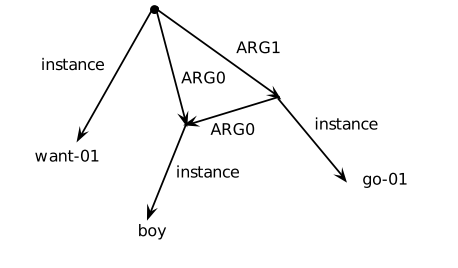
\includegraphics[width=7cm]{images/amr-boy.png}
\end{center}
\caption{\labfig{amr-boy}Graph visualization of the AMR structure associated with the sentence "The boy wants to go.". Figure extracted from \textcite{banarescu2013abstract}.}
\end{figure}

% \paragraph{Abstract Meaning Representations (AMR)} is a semantic representation language. AMR graphs are rooted, labeled, directed, acyclic graphs (DAGs), comprising whole sentences. They are intended to abstract away from syntactic representations, in the sense that sentences which are similar in meaning should be assigned the same AMR, even if they are not identically worded. By nature, the AMR language is biased towards English – it is not meant to function as an international auxiliary language.

% Abstract Meaning Representations have originally been introduced by Langkilde and Knight (1998) as a derivation from the Penman Sentence Plan Language, they are thus continuing a long tradition in Natural Language Generation and this has been their original domain of application. AMRs have re-gained attention since \textcite{banarescu2013abstract} in particular, this includes the extension to novel tasks such as machine translation and natural language understanding. The modern (post-2010) AMR format preserves the syntax and many syntactic conceptions of the original AMR format but has been thoroughly revised to better align with PropBank. Moreover, AMR has been extended with formal conventions for metadata and conventions for entity linking (here, linking with Wikipedia entries).

% Existing AMR technology includes tools and libraries for parsing, visualization, and surface generation as well as a considerable number of publicly available data sets. Many of these resources are collected at the AMR homepage\sidenote{\url{https://amr.isi.edu/}} at ISI/USC where AMR technology has been originally developed.

% Example sentence: The boy wants to go.

% \texttt{(h\,/\,hug-01
%     \\ \T :ARG0\,(b\,/\,boy)
%     \\ \T :ARG1\,(d\,/\,dog))}
    
% % (w / want-01
% %   :arg0 (b / boy)
% %   :arg1 (g / go-01
% %     :arg0 b))

% As far as predicate semantics are concerned, the role inventory of PropBank is largely based on semantic role annotations in the style of PropBank. Note that in pre-2010 AMR format, `:arg0` would be `:agent`, etc.

% \textcite{banarescu2013abstract} claim that this is equivalent to the following logical formula:

% \begin{equation}
% \exists w,b,g:instance(w,want\_01)\wedge instance(g,go\_01)\wedge instance(b,boy)\wedge arg0(w,b)\wedge arg1(w,g)\wedge arg0(g,b)
% % \exists w,b,g:instance(w,want\_01)\wedge instance(g,go\_01)\wedge instance(b,boy)\wedge arg0(w,b)\wedge arg1(w,g)\wedge arg0(g,b)
% \end{equation}

% In addition, they claim that this representation makes the will of the boy more explicit, highlighting that the intention of the boy is that he himself goes away (because `want-01` is the type of the top-level predicate).

\paragraph{Universal Conceptual Cognitive Annotation (UCCA)} is a semantic representation based on directed acyclic graphs \parencite{abend2013universal}. Terminal nodes can be arbitrary morphemes, words, or multi-word chunks. Inner nodes consist of a single entity defined by semantic or cognitive factors over the connected units. Edge labels represent a child's contribution to the semantics of the parent unit. The annotated text is mostly based on English Wikipedia articles with 148 annotated passages  (an average length of 385 tokens).

\paragraph{Discourse Representation Structures (DRS)} are formal meaning representations developed as part of the Discourse Representation Theory (DRT) \parencite{kamp1993discourse}. It aims at better-representing phenomena such as interactions between indefinite noun phrases and (anaphoric) pronouns, treatment of negation, modals, and quantification scope. The specificity of DRT is to propose an interpretation of discourses spanning over more than one sentence and not only individual sentences. It proposes a view of language where its interaction with its context defines the semantics of a sentence. The framework presents similarities with logical formalisms as it enables the evaluation of a sentence's truth value and performs semantic inference. Regarding the representation structure, DRS map the discourse to a graph where nodes are discourse referents representing entities under discussion and edges representing information exchanged between referents.
% itself, it is more related to \bcomment{AMR}{not really. DRT can be seen as a notation for first order logic}. 
%TODO Comparer avec logic? C.f. wikipedia ?

% \paragraph{Frame semantic parsing} The FrameNet project\sidenote{\url{https://framenet.icsi.berkeley.edu/}} is building a lexical database of English that is both human- and machine-readable, based on annotating examples of how words are used in actual texts. From the student's point of view, it is a dictionary of more than 13,000 word senses, most of them with annotated examples that show the meaning and usage. For the researcher in Natural Language Processing, the more than 200,000 manually annotated sentences linked to more than 1,200 semantic frames provide a unique training dataset for semantic role labeling, used in applications such as information extraction, machine translation, event recognition, sentiment analysis, etc. For students and teachers of linguistics it serves as a valence dictionary, with uniquely detailed evidence for the combinatorial properties of a core set of the English vocabulary. The project has been in operation at the International Computer Science Institute in Berkeley since 1997, supported primarily by the National Science Foundation, and the data is freely available for download. It has been downloaded and used by researchers around the world for a wide variety of purposes (see FrameNet downloaders). FrameNet-like databases have been built for a number of languages (see FrameNets in other languages) and a new project is working on aligning the FrameNets across languages.

\paragraph{Semantic Dependency Parsing (SDP)} is a formal meaning representation in the form of a directed graph with arcs between pairs of words \parencite{oepen_15}. The vertices between words describe predicate-argument relationships. 

\subsection{Programming languages}

% \paragraph{SQL parsing}
Finally, as mentioned in the survey conducted in \textcite{kamath_19}, a line of work aims at translating natural language into executable functions from general-purpose programming languages. Such languages have an explicit syntax and are less subject to ambiguity. Many benchmarks exist, in particular, to convert questions into executable SQL queries \parencite{dahl_94, radev_18}.

% Distributional semantic representations
\section{Practical limits of symbolic representations}
\labsec{meaning:distributional}

The methods presented above represent meaning in the form of dedicated structures. Such frameworks have explicit properties which facilitate their use. For example, SQL queries can be executed on a knowledge base to answer factual questions. However, meaning representations are usually supposed to label a training dataset to learn the mapping of the sentences. Labeling such a dataset is usually complex and requires linguistic experts. The process should be repeated for every domain and language and is usually restricted to generic English data. Finally, the semantic parser is not guaranteed to produce the proper structure and may be subject to errors.

% \bcomment{remove the quote, it is incorrect: slp3 is not 2009. CIte 2022, forth-comming}{}
On the other hand, distributional semantic representations propose to represent semantic meaning in the form of a real-value fixed-length vector \parencite{jurafsky_2009}.\sidenote{\url{https://web.stanford.edu/~jurafsky/slp3/6.pdf}} As for formal representations, many methods exist to learn this mapping. However, the main idea is to use self-supervised data that do not require heavy labeling effort. In this perspective, we learn to map a sentence to a semantic vector using only the structure and patterns within raw text. In particular, we train such methods to verify specific sub-properties induced by natural language understanding, such as predicting inference or reconstructing a sentence surface form given its embedding. In this work, we will focus on such approaches, and we will provide an in-depth review of such methods in \refch{training}.

% Rather than learning a mapping from text to meaning representations, we can make sure that such representations verify specific sub-properties. \textcite{jurafsky_2009}\sidenote{https://web.stanford.edu/~jurafsky/slp3/6.pdf}

% This time representation more simple : a vector every time. Not like formal representation with very different structures. But there is many different architectures to compose words into sentence representations and get this vector.

% Distributional semantic, vector space